\documentclass[journal,12pt,twocolumn]{IEEEtran}

\usepackage{setspace}
\usepackage{gensymb}
\singlespacing
\usepackage[cmex10]{amsmath}

\usepackage{amsthm}

\usepackage{mathrsfs}
\usepackage{txfonts}
\usepackage{stfloats}
\usepackage{bm}
\usepackage{cite}
\usepackage{cases}
\usepackage{subfig}

\usepackage{longtable}
\usepackage{multirow}

\usepackage{enumitem}
\usepackage{mathtools}
\usepackage{steinmetz}
\usepackage{tikz}
\usepackage{circuitikz}
\usepackage{verbatim}
\usepackage{tfrupee}
\usepackage[breaklinks=true]{hyperref}
\usepackage{graphicx}
\usepackage{tkz-euclide}

\usetikzlibrary{calc,math}
\usepackage{listings}
    \usepackage{color}                                            %%
    \usepackage{array}                                            %%
    \usepackage{longtable}                                        %%
    \usepackage{calc}                                             %%
    \usepackage{multirow}                                         %%
    \usepackage{hhline}                                           %%
    \usepackage{ifthen}                                           %%
    \usepackage{lscape}     
\usepackage{multicol}
\usepackage{chngcntr}

\DeclareMathOperator*{\Res}{Res}

\renewcommand\thesection{\arabic{section}}
\renewcommand\thesubsection{\thesection.\arabic{subsection}}
\renewcommand\thesubsubsection{\thesubsection.\arabic{subsubsection}}

\renewcommand\thesectiondis{\arabic{section}}
\renewcommand\thesubsectiondis{\thesectiondis.\arabic{subsection}}
\renewcommand\thesubsubsectiondis{\thesubsectiondis.\arabic{subsubsection}}


\hyphenation{op-tical net-works semi-conduc-tor}
\def\inputGnumericTable{}                                 %%

\lstset{
%language=C,
frame=single, 
breaklines=true,
columns=fullflexible
}
\begin{document}


\newtheorem{theorem}{Theorem}[section]
\newtheorem{problem}{Problem}
\newtheorem{proposition}{Proposition}[section]
\newtheorem{lemma}{Lemma}[section]
\newtheorem{corollary}[theorem]{Corollary}
\newtheorem{example}{Example}[section]
\newtheorem{definition}[problem]{Definition}

\newcommand{\BEQA}{\begin{eqnarray}}
\newcommand{\EEQA}{\end{eqnarray}}
\newcommand{\define}{\stackrel{\triangle}{=}}
\bibliographystyle{IEEEtran}
\raggedbottom
\setlength{\parindent}{0pt}
\providecommand{\mbf}{\mathbf}
\providecommand{\pr}[1]{\ensuremath{\Pr\left(#1\right)}}
\providecommand{\qfunc}[1]{\ensuremath{Q\left(#1\right)}}
\providecommand{\sbrak}[1]{\ensuremath{{}\left[#1\right]}}
\providecommand{\lsbrak}[1]{\ensuremath{{}\left[#1\right.}}
\providecommand{\rsbrak}[1]{\ensuremath{{}\left.#1\right]}}
\providecommand{\brak}[1]{\ensuremath{\left(#1\right)}}
\providecommand{\lbrak}[1]{\ensuremath{\left(#1\right.}}
\providecommand{\rbrak}[1]{\ensuremath{\left.#1\right)}}
\providecommand{\cbrak}[1]{\ensuremath{\left\{#1\right\}}}
\providecommand{\lcbrak}[1]{\ensuremath{\left\{#1\right.}}
\providecommand{\rcbrak}[1]{\ensuremath{\left.#1\right\}}}
\theoremstyle{remark}
\newtheorem{rem}{Remark}
\newcommand{\sgn}{\mathop{\mathrm{sgn}}}
\providecommand{\abs}[1]{\left\vert#1\right\vert}
\providecommand{\res}[1]{\Res\displaylimits_{#1}} 
\providecommand{\norm}[1]{\left\lVert#1\right\rVert}
%\providecommand{\norm}[1]{\lVert#1\rVert}
\providecommand{\mtx}[1]{\mathbf{#1}}
\providecommand{\mean}[1]{E\left[ #1 \right]}
\providecommand{\fourier}{\overset{\mathcal{F}}{ \rightleftharpoons}}
%\providecommand{\hilbert}{\overset{\mathcal{H}}{ \rightleftharpoons}}
\providecommand{\system}{\overset{\mathcal{H}}{ \longleftrightarrow}}
	%\newcommand{\solution}[2]{\textbf{Solution:}{#1}}
\newcommand{\solution}{\noindent \textbf{Solution: }}
\newcommand{\cosec}{\,\text{cosec}\,}
\providecommand{\dec}[2]{\ensuremath{\overset{#1}{\underset{#2}{\gtrless}}}}
\newcommand{\myvec}[1]{\ensuremath{\begin{pmatrix}#1\end{pmatrix}}}
\newcommand{\mydet}[1]{\ensuremath{\begin{vmatrix}#1\end{vmatrix}}}
\numberwithin{equation}{subsection}

\makeatletter
\@addtoreset{figure}{problem}
\makeatother
\let\StandardTheFigure\thefigure
\let\vec\mathbf

\renewcommand{\thefigure}{\theproblem}

\def\putbox#1#2#3{\makebox[0in][l]{\makebox[#1][l]{}\raisebox{\baselineskip}[0in][0in]{\raisebox{#2}[0in][0in]{#3}}}}
     \def\rightbox#1{\makebox[0in][r]{#1}}
     \def\centbox#1{\makebox[0in]{#1}}
     \def\topbox#1{\raisebox{-\baselineskip}[0in][0in]{#1}}
     \def\midbox#1{\raisebox{-0.5\baselineskip}[0in][0in]{#1}}
\vspace{3cm}
\title{Assignment 8}
\author{Sachinkumar Dubey - EE20MTECH11009}
\maketitle
\newpage
\bigskip
\renewcommand{\thefigure}{\theenumi}
\renewcommand{\thetable}{\theenumi}
Download all python codes from 
\begin{lstlisting}
https://github.com/sachinomdubey/Matrix-theory/Assignment8/codes
\end{lstlisting}
%
and latex-tikz codes from 
%
\begin{lstlisting}
https://github.com/sachinomdubey/Matrix-theory/Assignment8
\end{lstlisting}
\section{Problem}
(Dresden/Page80/Example1/D)\\Determine the distances of the point $D(-1, 2, -4)$ from the plane:
\begin{align}
3x+2y-6z-2=0\label{eq:1.0.1}
\end{align}
\section{Solution}
Equation of plane can be written in the form: 
\begin{align}\label{eq1}
	\vec{n}^T\vec{x} &= c
\end{align}
Writing the given plane equation \eqref{eq:1.0.1} in the form \eqref{eq1}:
\begin{align}\label{eq2}
	\myvec{3 & 2 & -6}\myvec{x\\y\\z} &= 2
\intertext{Where,}
    \vec{n} &= \myvec{3\\2\\-6} \\
    \vec{x} &= \myvec{x\\y\\z}  \quad  c = 2
\end{align}
A vector from the plane to the point $D(-1, 2, -4)$ is given by:
\begin{align}
\vec{w}=\vec{D}-\vec{x}
\intertext{Where,}
    \vec{D} &= \myvec{-1\\2\\-4} \\
    \vec{x} &= \myvec{x\\y\\z} 
\end{align}
The projection of $\vec{w}$ onto the normal vector $\vec{n}$ can be written as:
\begin{align}
    \text{proj}_\vec{n}\vec{w}=\frac{\vec{n}^T\vec{w}}{\vec{n}^T\vec{n}}\cdot\vec{n}\\
    \text{proj}_\vec{n}\vec{w}=\frac{\vec{n}^T(\vec{D}-\vec{x})}{\vec{n}^T\vec{n}}\cdot\vec{n}\\
     \text{proj}_\vec{n}\vec{w}=\frac{\vec{n}^T\vec{D}-\vec{n}^T\vec{x}}{\vec{n}^T\vec{n}}\cdot\vec{n}\\
\end{align}
From equation \eqref{eq1},
\begin{align}
     \text{proj}_\vec{n}\vec{w}=\frac{\vec{n}^T\vec{D}-c}{\vec{n}^T\vec{n}}\cdot\vec{n}\\
\end{align}
Putting the values of $\vec{n}$, $\vec{D}$ and $c$, we get:
\begin{align}
     \text{proj}_\vec{n}\vec{w}=\frac{\myvec{3&2&-6}\myvec{-1\\2\\-4} -2}{\myvec{3&2&-6}\myvec{3\\2\\-6}}\cdot\myvec{3\\2\\-6}\\
      \text{proj}_\vec{n}\vec{w}=\frac{23}{49}\cdot\myvec{3\\2\\-6}
\end{align}
The distance $d_{min}$ between point $D(-1, 2, -4)$ and the given plane  is obtained as:
\begin{align}
    d_{min}=\norm{\text{proj}_\vec{n}\vec{w}}\\
    d_{min}=\frac{23}{49}\cdot\norm{\myvec{3\\2\\-6}}
\end{align}
\begin{align}
    \therefore d_{min}=\frac{23}{49} \times \sqrt{(3)^2+(2)^2+(-6)^2}\\
    \therefore d_{min}=\frac{23}{49} \times 7\\
    \implies \boxed{d_{min}=\frac{23}{7}= 3.2857}
\end{align}
\begin{figure}[h!]
\centering
\resizebox{\columnwidth}{!}
    {
    


\tikzset{every picture/.style={line width=0.75pt}} %set default line width to 0.75pt        

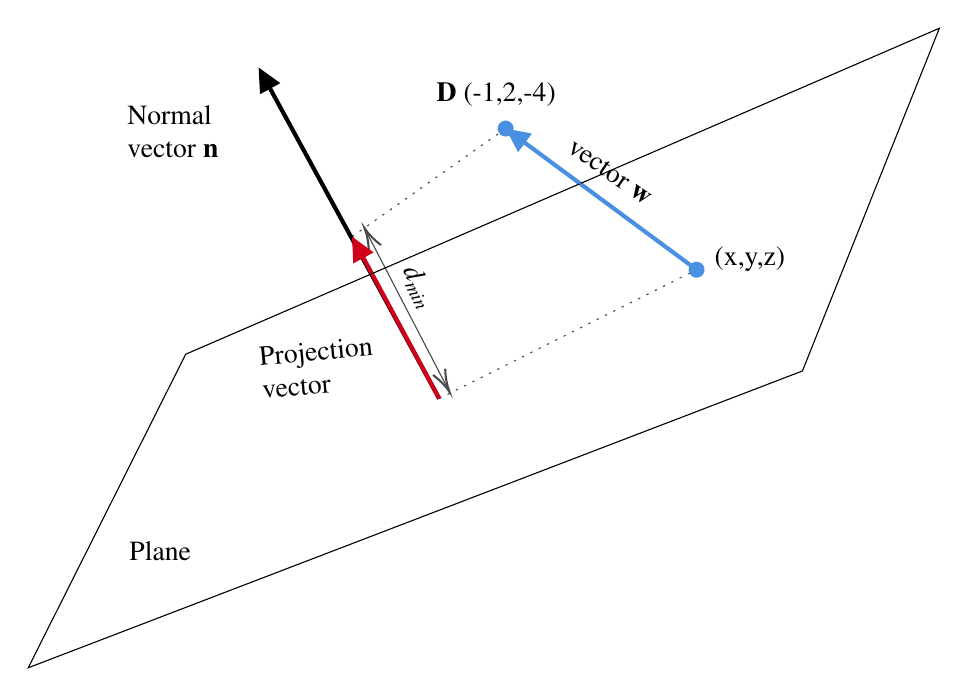
\begin{tikzpicture}[x=0.75pt,y=0.75pt,yscale=-1,xscale=1]
%uncomment if require: \path (0,324); %set diagram left start at 0, and has height of 324

%Straight Lines [id:da012474511036709712] 
\draw [color={rgb, 255:red, 74; green, 74; blue, 74 }  ,draw opacity=1 ] [dash pattern={on 0.84pt off 2.51pt}]  (165.51,108.36) -- (239.51,56.27) ;
%Straight Lines [id:da164610693713777] 
\draw [color={rgb, 255:red, 74; green, 74; blue, 74 }  ,draw opacity=1 ] [dash pattern={on 0.84pt off 2.51pt}]  (207.51,186.36) -- (331.51,124.27) ;
%Straight Lines [id:da0009900971082483778] 
\draw [color={rgb, 255:red, 74; green, 74; blue, 74 }  ,draw opacity=1 ]   (211.58,181.43) -- (172.42,105.98) ;
\draw [shift={(171.5,104.2)}, rotate = 422.57] [color={rgb, 255:red, 74; green, 74; blue, 74 }  ,draw opacity=1 ][line width=0.75]    (10.93,-3.29) .. controls (6.95,-1.4) and (3.31,-0.3) .. (0,0) .. controls (3.31,0.3) and (6.95,1.4) .. (10.93,3.29)   ;
\draw [shift={(212.5,183.2)}, rotate = 242.57] [color={rgb, 255:red, 74; green, 74; blue, 74 }  ,draw opacity=1 ][line width=0.75]    (10.93,-3.29) .. controls (6.95,-1.4) and (3.31,-0.3) .. (0,0) .. controls (3.31,0.3) and (6.95,1.4) .. (10.93,3.29)   ;
%Straight Lines [id:da6317108471264852] 
\draw [line width=1.5]    (207.51,186.36) -- (122.42,30.38) ;
\draw [shift={(120.51,26.87)}, rotate = 421.39] [fill={rgb, 255:red, 0; green, 0; blue, 0 }  ][line width=0.08]  [draw opacity=0] (11.61,-5.58) -- (0,0) -- (11.61,5.58) -- cycle    ;
%Straight Lines [id:da4711513779445873] 
\draw [color={rgb, 255:red, 74; green, 144; blue, 226 }  ,draw opacity=1 ][line width=1.5]    (331.51,124.27) -- (242.72,58.64) ;
\draw [shift={(239.51,56.27)}, rotate = 396.47] [fill={rgb, 255:red, 74; green, 144; blue, 226 }  ,fill opacity=1 ][line width=0.08]  [draw opacity=0] (11.61,-5.58) -- (0,0) -- (11.61,5.58) -- cycle    ;
%Straight Lines [id:da281513313013386] 
\draw [color={rgb, 255:red, 208; green, 2; blue, 27 }  ,draw opacity=1 ][line width=1.5]    (207.51,186.36) -- (167.4,111.89) ;
\draw [shift={(165.51,108.36)}, rotate = 421.7] [fill={rgb, 255:red, 208; green, 2; blue, 27 }  ,fill opacity=1 ][line width=0.08]  [draw opacity=0] (11.61,-5.58) -- (0,0) -- (11.61,5.58) -- cycle    ;
%Shape: Polygon [id:ds23253650680866844] 
\draw   (85.38,164.99) -- (448.5,7.93) -- (382.5,173.07) -- (9.5,316.07) -- (9.5,316.07) -- cycle ;
%Straight Lines [id:da02842289374539675] 
\draw [color={rgb, 255:red, 74; green, 144; blue, 226 }  ,draw opacity=1 ]   (239.51,56.27) -- (331.51,124.27) ;
\draw [shift={(331.51,124.27)}, rotate = 36.47] [color={rgb, 255:red, 74; green, 144; blue, 226 }  ,draw opacity=1 ][fill={rgb, 255:red, 74; green, 144; blue, 226 }  ,fill opacity=1 ][line width=0.75]      (0, 0) circle [x radius= 3.35, y radius= 3.35]   ;
\draw [shift={(239.51,56.27)}, rotate = 36.47] [color={rgb, 255:red, 74; green, 144; blue, 226 }  ,draw opacity=1 ][fill={rgb, 255:red, 74; green, 144; blue, 226 }  ,fill opacity=1 ][line width=0.75]      (0, 0) circle [x radius= 3.35, y radius= 3.35]   ;

% Text Node
\draw (56,44) node [anchor=north west][inner sep=0.75pt]   [align=left] {Normal \\vector \textbf{n} };
% Text Node
\draw (118.97,160.37) node [anchor=north west][inner sep=0.75pt]  [rotate=-354.79] [align=left] {Projection \\vector};
% Text Node
\draw (205,33) node [anchor=north west][inner sep=0.75pt]   [align=left] {\textbf{D }(-1,2,-4)};
% Text Node
\draw (339,112) node [anchor=north west][inner sep=0.75pt]   [align=left] {(x,y,z)};
% Text Node
\draw (272.66,59.12) node [anchor=north west][inner sep=0.75pt]  [rotate=-34.52] [align=left] {vector \textbf{w} };
% Text Node
\draw (198.69,119.24) node [anchor=north west][inner sep=0.75pt]  [rotate=-64.65] [align=left] {$d_{min}$};
% Text Node
\draw (57,254.07) node [anchor=north west][inner sep=0.75pt]   [align=left] {Plane};


\end{tikzpicture}

    }
    \caption{Distance between a point and a plane}
\end{figure}
\end{document}